
%%%%%%%%%%%%%%%%%%%%%%%%%%%%%%%%%%%%%%%%%%%%%%%%%%%%%%%%%%%%%%%%%%%%%%%%%%%%%%%%%%
\chapter{DUNE Science}
\label{v1ch:science}

\section{Overview} % Anne added new 5/8

This chapter summarizes DUNE's potential for achieving its core
physics objectives based on the current %understanding of the 
experimental landscape, scenarios for staging \fixme{LBNF and} DUNE, and 
the technical capabilities of DUNE at each stage. \fixme{The objectives include topics in long-baseline neutrino 
physics, nucleon decay, supernova neutrinos, astrophysics and short-baseline physics.}
A detailed description of the physics objectives of DUNE is provided in
the main text of this document. \fixme{reference chap or sec} 

\fixme{This next part seems like it should be in the Strategy chapter and just referenced here. You could keep something about improvements in systematic uncertainties. Start Anne's }

The \ktadj{40} DUNE far detector (FD) is expected to
be built as four \ktadj{10} modules, which will come online over the course
of several years.  The near detector (ND) will likely start operations
after FD operations are already ongoing.  Without any ND constraints,
systematic uncertainties will be larger in the early stages of the
experiment. Additionally, the LBNF beam power is expected to be upgraded
from $\sim$\SI{1}\MW{} to $\sim$\SI{2}\MW{} during the course of the experiment. 
The staging strategy is described in Chapter~\ref{v1ch:strategy}. 
It is assumed that data sets collected during earlier stages can be reanalyzed with new
assumptions, so that each improvement in systematic uncertainty is applied
to the full exposure up to that point.

\fixme{end Anne's; suggestion to go straight to next section.}

In the DUNE project, the \ktadj{40} DUNE far detector (FD) is expected to
be built as four \ktadj{10} modules, which will come online over the course
of several years.  The near detector (ND) will likely start operations
after FD operations are already ongoing.  Without any ND constraints,
systematic uncertainties will be larger in the early stages of the
experiment. Additionally, the LBNF beam power is expected to be upgraded
from $\sim$\SI{1}\MW{} to $\sim$\SI{2}\MW{} during the course of the experiment. For
a rough estimate of the sensitivity of DUNE as a function of real time
for the first \num{10} years of operation, the following staging plan has
been assumed:
\begin{itemize}
 \item Year 1: \SI{10}\kt{} FD mass; \SI{1.07}\MW{} beam power; No ND constraints (assume \num{5}\% signal systematic)
 \item Year 2: Add second \ktadj{10} FD module, for a total FD mass of \SI{20}\kt
 \item Year 3: Add third \ktadj{10} FD module, for a total FD mass of \SI{30}\kt; Include constraints from preliminary ND data analysis (assume \num{3}\% signal systematic)
 \item Year 4: Add fourth \ktadj{10} FD module, for a total FD mass of \SI{40}\kt
 \item Year 5: Include constraints from a full ND data analysis (assume \num{2}\% signal systematic)
 \item Year 7: Upgrade of beam power to \SI{2.14}\MW
\end{itemize}
It is assumed that previous data sets can be reanalyzed with new
assumptions, so each improvement in systematic uncertainty is applied
to the full exposure up to that point.

%Add that integrated exposure is 535 kt-MW-yr after 10 years?

%%%%%%%%%%%%%%%%%%%%%%%%%%%%%%%%%%%%%%%%%%%%%%%%%%%%%%%%%%%%%%%%%%%%%%%%%%%%%%%%%%
\section{Neutrino Mixing, Mass Hierarchy and CP Violation}
%\subsection{Long-Baseline/Oscillation Physics}

\fixme{Title puts MH 2nd, then it's the first thing you see in the text; a little strange. I suggest getting rid of these would-be headings.}

\textbf{Neutrino Mass Hierarchy:} The \SIadj{1300}{\km} baseline
establishes one of DUNE's key strengths: sensitivity to the matter
effect. This effect leads to a large discrete asymmetry in the
\numu $\to$ \nue versus \anumu $\to$ \anue
%$\nu_\mu\to \nu_e$ versus $\overline{\nu}_\mu \to \overline{\nu}_e$
oscillation probabilities, the sign of which depends on the mass
hierarchy (MH).  At 1300~km this asymmetry is approximately
$\pm 40\%$ in the region of the peak flux; this is larger than the
maximal possible CP-violating asymmetry associated with \deltacp,
meaning that both the MH and \deltacp can be
determined unambiguously with high confidence within the same
experiment using the beam neutrinos.
%\fixme{I would drop `using the beam neutrinos'}
% a feat unattainable for an experiment at a much shorter baseline.  

In detail, the sensitivity of DUNE depends on the actual values of
poorly known mixing parameters (mainly \deltacp and
\sinst{23}), %$\sin^2{\theta_{23}}$), 
as well as the true value of the MH itself.
The discrimination between the two MH hypotheses is characterized as a
function of the \emph{a priori} unknown true value of \deltacp by
considering the difference, denoted $\Delta \chi^2$, between the
$-2\log{\cal L}$ values calculated for a data set with respect to
these hypotheses, considering all possible values of
\deltacp\footnote{For the case of the MH determination, the usual
  association of this test statistic with a $\chi^2$ distribution for
  one degree of freedom is incorrect; additionally the assumption of a
  Gaussian probability density % added 'a'
  implicit in this notation is not exact.  The discussion in
  Chapter~3 of \volphys provides a brief description of the
  statistical considerations.}.  In terms of this test statistic, the
MH sensitivity of DUNE with an exposure of \SI{300}\ktMWyr{}  which
corresponds to seven years of data (\num{3.5} years in neutrino mode plus
\num{3.5} years in antineutrino mode) with a \ktadj{10} detector and a \SI{1.07}\MW{}
beam is illustrated in Figure~\ref{fig:mhexec} for the case of normal
hierarchy and the current best fit value of \sinst{23} = \SI{45}. %$\sin^2 \theta_{23} = 0.45$.
%
\begin{cdrfigure}[Summary of mass hierarchy sensitivities]{mhexec}{The
    square root of the mass hierarchy discrimination metric $\Delta
    \chi^2$ is plotted as a function of the unknown value of \deltacp
    for an exposure of \SI{300}\ktMWyr{} % ~kt-MW-yr 
    (left).  The minimum significance
    --- the lowest point on the curve on the left - with which the mass
    hierarchy can be determined for all values of \deltacp as a
    function of years of exposure assuming the staging plan outlined in this chapter (right).
    The shaded region represents the range in sensitivity due to
    potential variations in the beam design.}
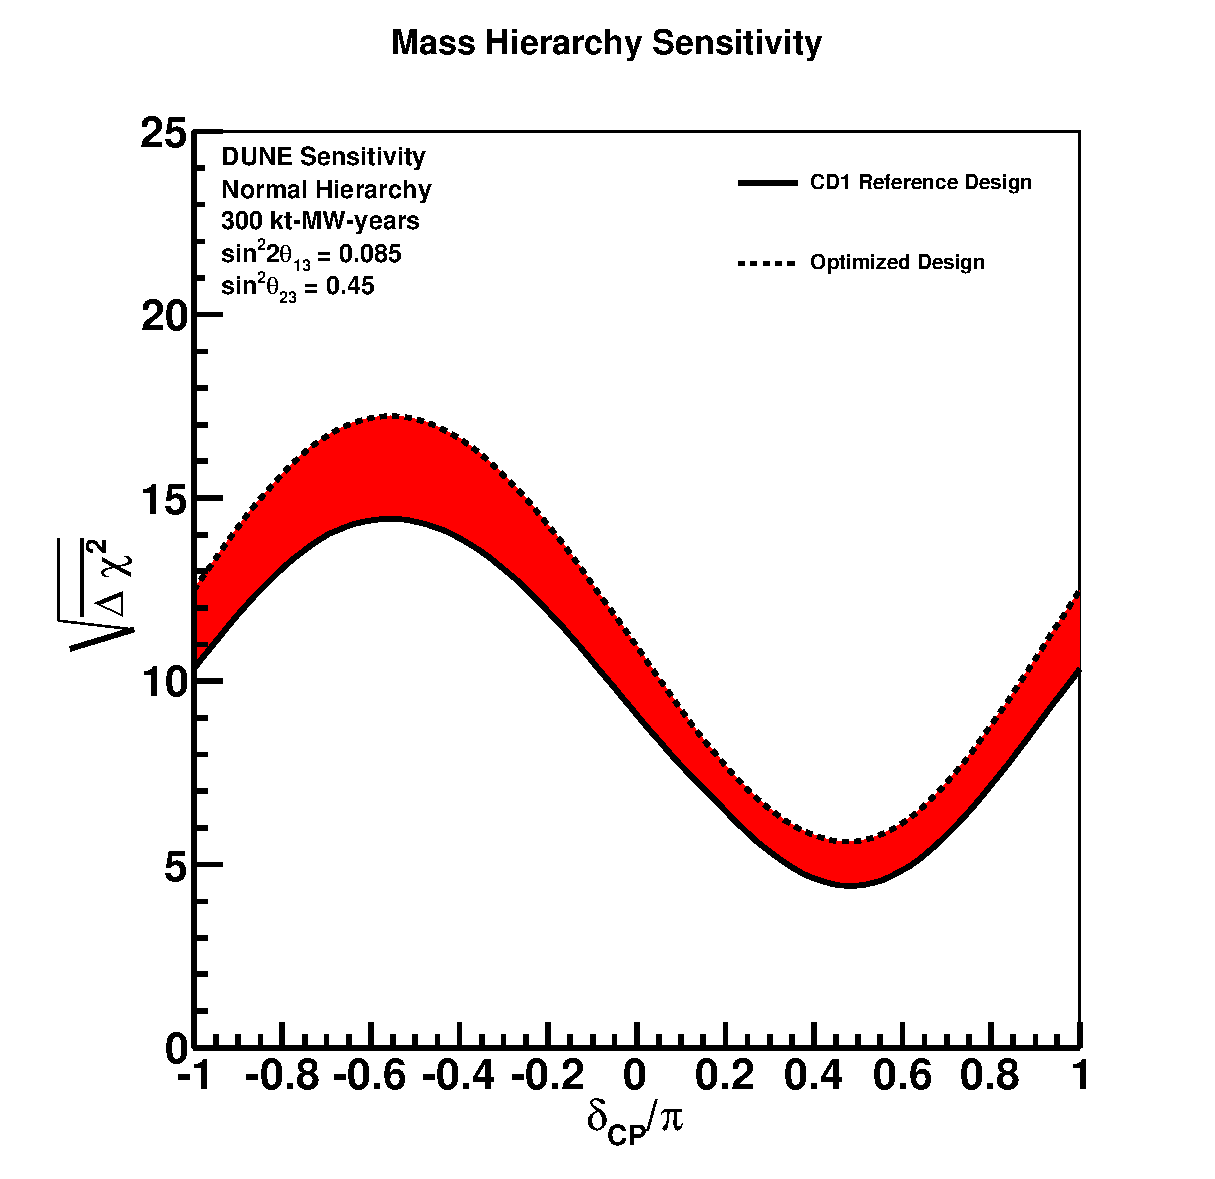
\includegraphics[width=0.49\textwidth]{volume-physics/figures/mh_300ktmwyear}
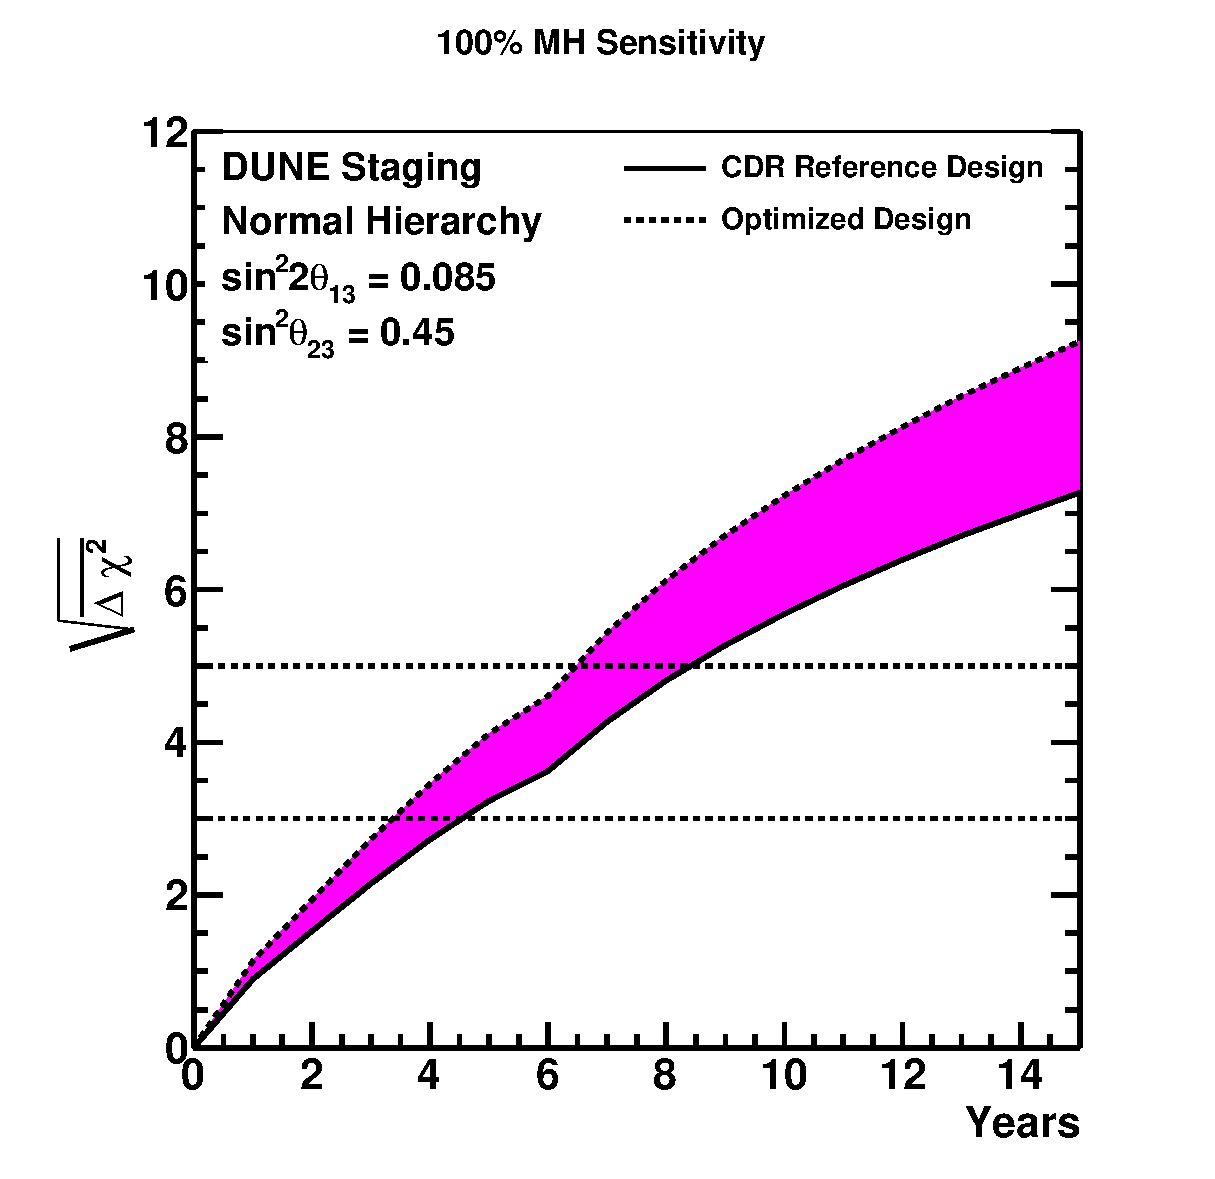
\includegraphics[width=0.49\textwidth]{volume-physics/figures/mh_exp_staging15yr}
\label{fig:mhexec}
\end{cdrfigure}

\fixme{staging plan may be moved to different chapter (two figure caption)} 
Across the overwhelming majority of the parameter space for the mixing
parameters that are not well known (mainly \deltacp and
\sinst{23}), DUNE's determination of the MH will be
definitive, but even for unfavorable combinations of the parameter
values, a statistically ambiguous outcome is highly unlikely.  The
least favorable scenario corresponds to a true value of \deltacp in
which the MH asymmetry is maximally offset by the leptonic CP
asymmetry, and where, independently, \sinst{23} takes on a
value at the low end of its experimentally allowed range.  For
this %worst-case
scenario, studies indicate that with the DUNE staging plan outlined earlier, the DUNE
LArTPC, operating for %ten years in a \SI{700}{\kW}
\num{8.5} years in the \GeVadj{80} \MWadj{1.07} (reference design) beam, 
can --- in a typical data set ---  distinguish between normal and inverted
hierarchy with $|\Delta \chi^2| = \overline{|\Delta \chi^2|} = 25$.
This corresponds to a $\geq 99.9996\%$ probability of determining the
correct hierarchy.  In $>97.5\%$ of data sets, DUNE will measure
$|\Delta \chi^2| > 9$ in this scenario, where measuring
$|\Delta\chi^2| = 9$ with an expected value of \num{25} corresponds to
a significance in excess of three Gaussian standard
deviations. Improvements to the beam design can lower the exposure
needed to reach this level of sensitivity from \SI{400}\ktMWyr{} to
around \SI{230}\ktMWyr. The dependence of the mass hierarchy
sensitivity on systematics is still under evaluation, but current
studies indicate a weak dependence on systematic uncertainties. This
indicates that a measurement of the unknown neutrino mass hierarchy
with very high precision can be carried out during the first few years
of operation with an optimized beamline design.

Concurrent analysis of the corresponding atmospheric-neutrino samples
in an underground detector will improve the precision and speed with
which the MH is resolved.

%It is important to note that for the
%initial stages of DUNE, a greatly improved level of precision in the
%determination of the MH can be achieved by incorporating
%constraints from NO$\nu$A and T2K data.  
%With an initial 10~kt detector, for half
%the range of possible \deltacp values, the expected significance 
%exceeds $\overline{\Delta \chi^2} = 25$; again this corresponds to a $\geq
%99.9996\%$ probability of determining the correct hierarchy.  To put
%this in context, it is notable that even an extended NO$\nu$A
%program~\cite{Messier:2013sfa} at four times its nominal exposure (of six
%years of operation at \SI{700}{\kW}), would have coverage at the
%$\overline{\Delta \chi^2} = 9$ level or better for only $40\%$ of the
%\deltacp range.

\textbf{CP Violation and the Measurement of {\boldmath \deltacp}:}
\fixme{Again, I suggest getting rid of this heading and rewording the first sentence in
the next pgraph to clearly introduce CP, i.e.,  ``With regard to
CP symmetry violation in the \numu to \nue oscillation channel, the DUNE program...''}

The DUNE program has two somewhat distinct objectives with regard to
CP symmetry violation in the $\nu_\mu \to \nu_e$ oscillation channel.
First, DUNE aims to make a precise determination of the value of
\deltacp within the context of the standard three-flavor mixing
scenario described by the PMNS neutrino mixing matrix.  Second, and perhaps more significantly,
DUNE aims to observe a signal for leptonic CP violation, independent
of the underlying nature of neutrino oscillation phenomenology.
Within the standard three-flavor mixing scenario, such a signal will
be observable, provided \deltacp is not too close to either of the
values for which there is no CP violation (zero and $\pi$).  Together,
the pursuit of these two goals provides a thorough test of the
standard three-flavor scenario.

Figure~\ref{fig:execsummaryCP} shows the expected sensitivity to CP
violation as well as the 1$\sigma$ resolution for \deltacp as a
function of exposure.  The exposure in detector mass (kiloton) $\times$ beam
power(MW) $\times$ time (years) required to measure $\delta_{\rm CP} = 0 $ with a
precision better than $10^\circ$ ranges from 290 to \SI{450}\ktMWyr{}
depending on the beam design.  
%At this beam power, in a six-year run,
%a \ktadj{10} far detector will be able to measure \deltacp to $\pm$
%20$^\circ$ $-$ 30$^\circ$ (depending on its value), independent of
%other experiments.
%This would be equivalent to a six-year run with a \SI{1.2}{\MW} beam.
A fully realized 
DUNE operating with multi-megawatt 
beam power can eventually achieve a precision 
comparable to the current precision on the CP phase in the
CKM matrix in the quark sector (5\%).
%
\begin{cdrfigure}[CP violation sensitivity and $\delta_{\rm CP}$
  resolution as a function of exposure]{execsummaryCP}{The
    significance with which CP violation can be determined for 75\% of
    \deltacp values as a function of exposure in years using the
    proposed staging plan outlined in this chapter (left). The
    expected 1$\sigma$ resolution for \deltacp as a function of
    exposure in \ktMWyr{} %kt-MW-years 
    (right). The shaded region represents the
    range in sensitivity due to potential variations in the beam
    design. This plot assumes normal mass hierarchy.}
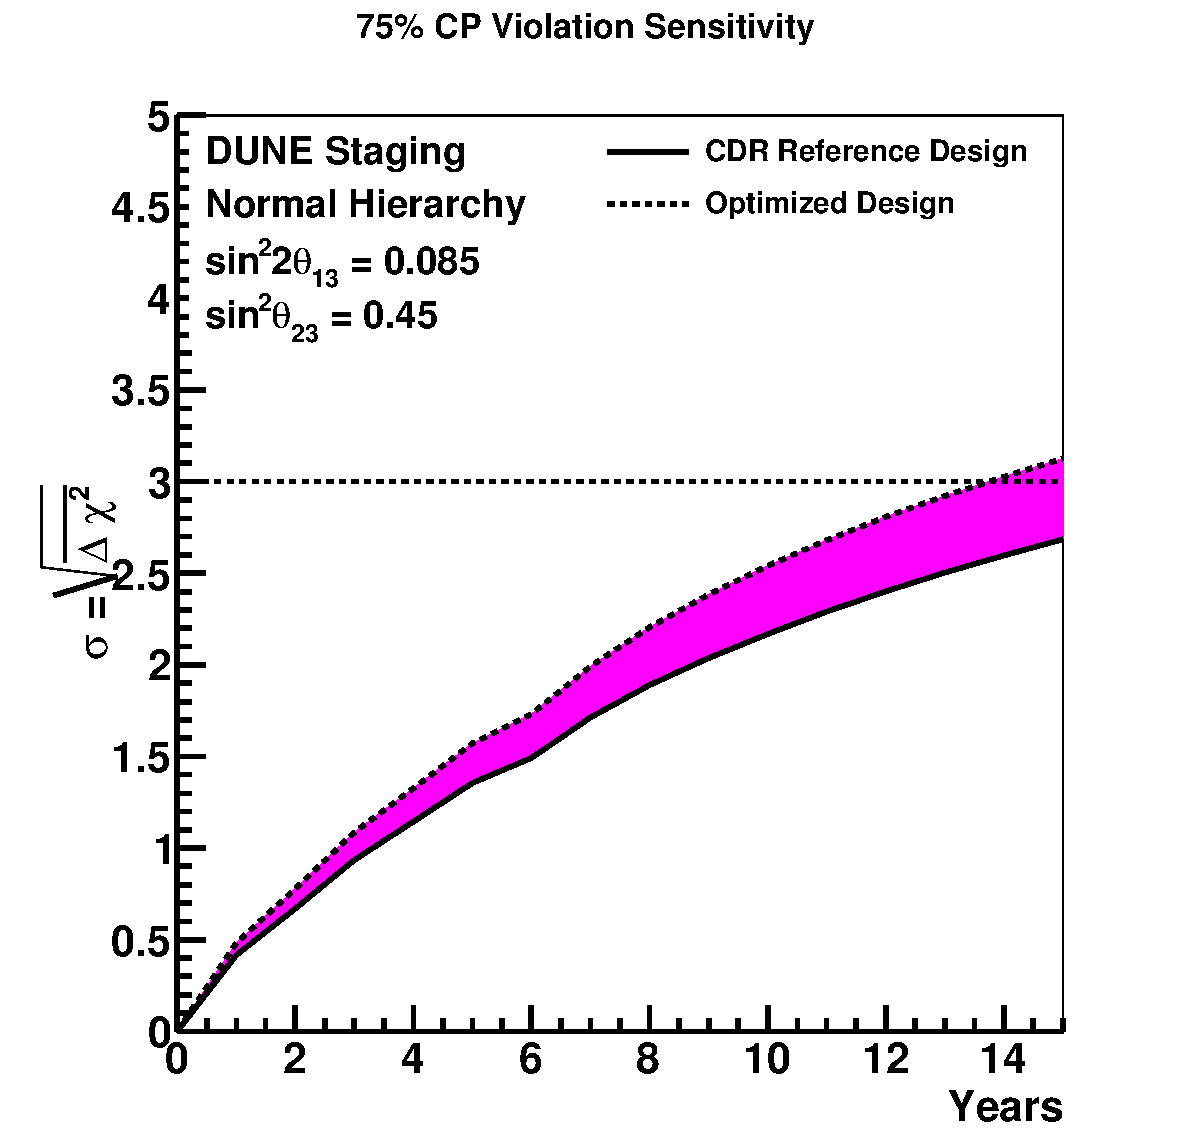
\includegraphics[width=0.49\textwidth]{volume-physics/figures/cpv75_exp_staging15yr}
 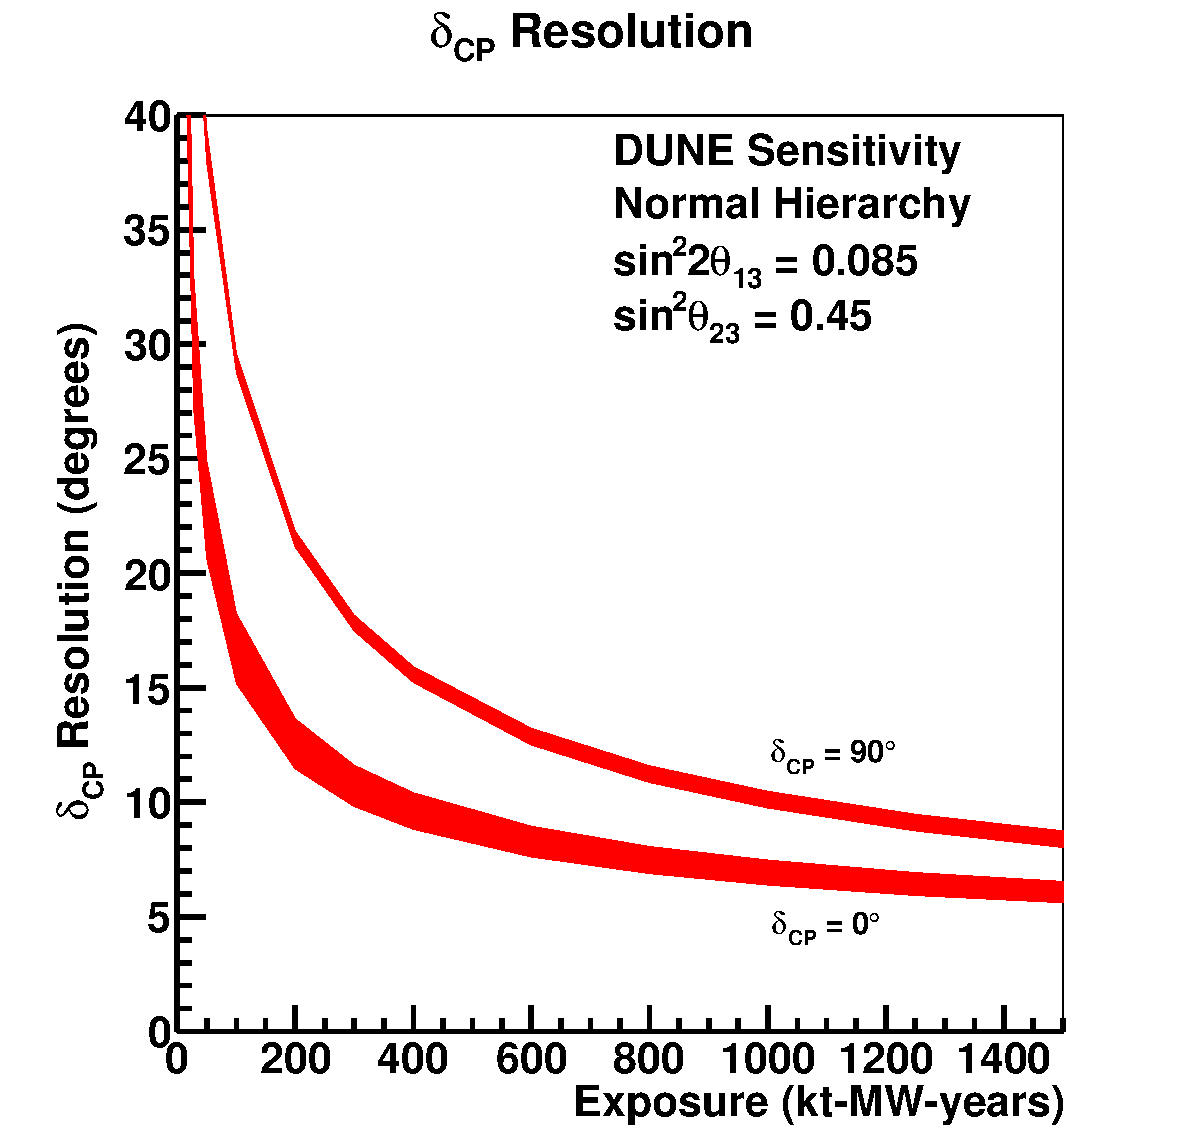
\includegraphics[width=0.49\textwidth]{volume-physics/figures/res_dcp_exp}
\end{cdrfigure}

To reach $5\sigma$ sensitivity for 50\% of the range of \deltacp, a
DUNE exposure in the range of \num{550} to \SI{810}\ktMWyr{}  is needed. The
range of exposures corresponds to potential variations in the beam
design, with the highest exposures corresponding to the reference beam
design. Table~\ref{tab:execosctable} summarizes the exposures needed to
achieve specific oscillation physics milestones.  The sensitivities
and exposures calculated are for the current best fit values of the
known neutrino mixing parameters. Changes in the value of
$\theta_{23}$ impact CP violation and mass hierarchy sensitivities the
most, as discussed in Volume 2, and can reduce or increase the exposure
needed to reach discovery potential for CP violation over a
significant fraction of \deltacp values. In addition, potential
improvements in beamline geometry, focusing and target element designs
that can significantly lower the exposure required for CP violation
discovery potential as demonstrated in Table~\ref{tab:execosctable}. Several such potential improvements are discussed
in CDR Volume 2 and Volume 3. A highly capable near neutrino detector
is required to control systematic uncertainties at a level lower than
the statistical uncertainties in the far detector needed to reach this
level of sensitivity.  No experiment can provide coverage at 100\% of
\deltacp values, since CP violation effects vanish as $\mdeltacp\to 0$
or $\pi$.

\textbf{\boldmath Determination of $\sin^2{2\theta_{23}}$ and Octant
  Resolution:} 
  \fixme{Again, remove the heading}
  
In long-baseline experiments with \numu beams, the
magnitude of \numu disappearance and \nue appearance signals is
proportional to \sinstt{23} and \sinst{23},
%$\sin^2{2\theta_{23}}$ and $\sin^2{\theta_{23}}$,
respectively, in the standard three-flavor mixing scenario.  Current
\numu disappearance data are consistent with close to maximal
mixing, $\theta_{23} = 45^\circ$.  To obtain the best sensitivity to
both the magnitude of its deviation from $45^\circ$ as well as its
sign ($\theta_{23}$ octant), a combined analysis of the two channels
is needed~\cite{Huber:2010dx}.  As demonstrated in Volume 2, a
\ktadj{40} DUNE detector with sufficient exposure will be able to
resolve the $\theta_{23}$ octant at the $3\sigma$ level or better for
$\theta_{23}$ values less than $43^\circ$ or greater than $48^\circ$.
A fully realized DUNE can measure $\theta_{23}$ with a precision of
$1^\circ$ or less, even for values within a few degrees of
$45^\circ$. Table~\ref{tab:execosctable} summarizes the exposures
needed to reach a given level of precision on the value of
$\theta_{23}$.

\begin{cdrtable}[Exposures needed to reach physics
  milestones]{lcc}{execosctable}{The exposure in mass (kt) $\times$ proton beam power
    (MW) $\times$ time (years) needed to reach certain oscillation physics
    milestones. The numbers are for normal hierarchy using the current best fit values of the known oscillation parameters. The two columns
    on the right are for different beam design assumptions. }
Physics milestone & Exposure \ktMWyr{} & Exposure \ktMWyr{}\\
  & (reference beam) & (optimized beam) \\ \toprowrule 
  $1^\circ$ $\theta_{23}$ resolution ($\theta_{23} = 42^\circ$) & 70  &  45\\ \colhline
  CPV at $3\sigma$ ($\delta_{\rm CP} = +\pi/2$)  & 70 & 60 \\ \colhline
  CPV at $3\sigma$ ($\delta_{\rm CP} = -\pi/2$)  & 160 & 100 \\ \colhline
  CPV at $5\sigma$ ($\delta_{\rm CP} = +\pi/2$)  & 280 & 210 \\ \colhline
  MH at  $5\sigma$ (worst point) & 400 & 230 \\ \colhline
  $10^\circ$ resolution ($\delta_{\rm CP} = 0$) & 450 & 290 \\ \colhline
  CPV at $5\sigma$ ($\delta_{\rm CP} = -\pi/2$)  & 525 & 320 \\ \colhline
  CPV at $5\sigma$ 50\% of \deltacp & 810 & 550 \\ \colhline 
  Reactor $\theta_{13}$ resolution ($\sin^2 2 \theta_{13} = 0.084 \pm 0.003$) & 1200 & 850 \\ \colhline
  CPV at $3\sigma$ 75\% of \deltacp & 1320 & 850\\ \colhline 

\end{cdrtable}


%%%%%%%%%%%%%%%%%%%%%%%%%%%%%%%%%%%%%%%%%%%%%%%%%%%%%%%%%%%%%%%%%%%%%%%%%%%%%%%%%%
%\paragraph*{Searches for Baryon Number Violation.}
\section{Nucleon Decay Physics Motivated by Grand Unified Theories}


The DUNE far detector will significantly extend lifetime sensitivity
for specific nucleon decay modes by virtue of its high detection
efficiency relative to water Cherenkov detectors and its low
background rates.  As an example, DUNE has enhanced capability for
detecting the $p\to K^+\bar{\nu}$ channel, where lifetime
predictions from supersymmetric models extend beyond, but remain close
to, the current (preliminary) Super-Kamiokande limit of $\tau/B >
\SI{5.9e33}{year}$ (90\% CL) from a \SI[number-unit-product = -,
inter-unit-product=\ensuremath{{}\cdot{}}]{260}{\kt\year}
exposure~\cite{kearns_isoups}\footnote{The lifetime shown here is
  divided by the branching fraction for this decay mode, $\tau/B$, and
  as such is a \emph{partial lifetime}.}.  The signature for an
isolated semi-monochromatic charged kaon in a LArTPC is distinctive,
with multiple levels of redundancy. 

The DUNE LArTPC far detectors deep underground will reach a limit of
\SI{3e34}{\year} after 10-12 years of operation
(Figure~\ref{fig:execsummarypdk}) depending on the deployment
scenario, and would see nine events with a background of 0.3 should
$\tau/B$ be \SI{1e34}{\year}, just beyond the current limit. A
\ktadj{40} detector will improve the current limits by an order of
magnitude after running for two decades. Even a \ktadj{10} detector
would yield an intriguing signal of a few events after a ten-year
exposure.


\begin{cdrfigure}[Sensitivity to the decay $p\to K^+ \bar{\nu}$
  with liquid argon detectors]{execsummarypdk} {Sensitivity to the
    decay $p\to K^+ \bar{\nu}$ as a function of time for different DUNE 
LArTPC module deployment strategies. 
  For comparison, the current limit from SK is also shown, as well as the projected limit from the proposed Hyper-K experiment with \SI{5600}\ktyr{} of exposure.
  The limits are at 90\% C.L., calculated for
  a Poisson process including background, assuming that the detected events
  equal the expected background.}
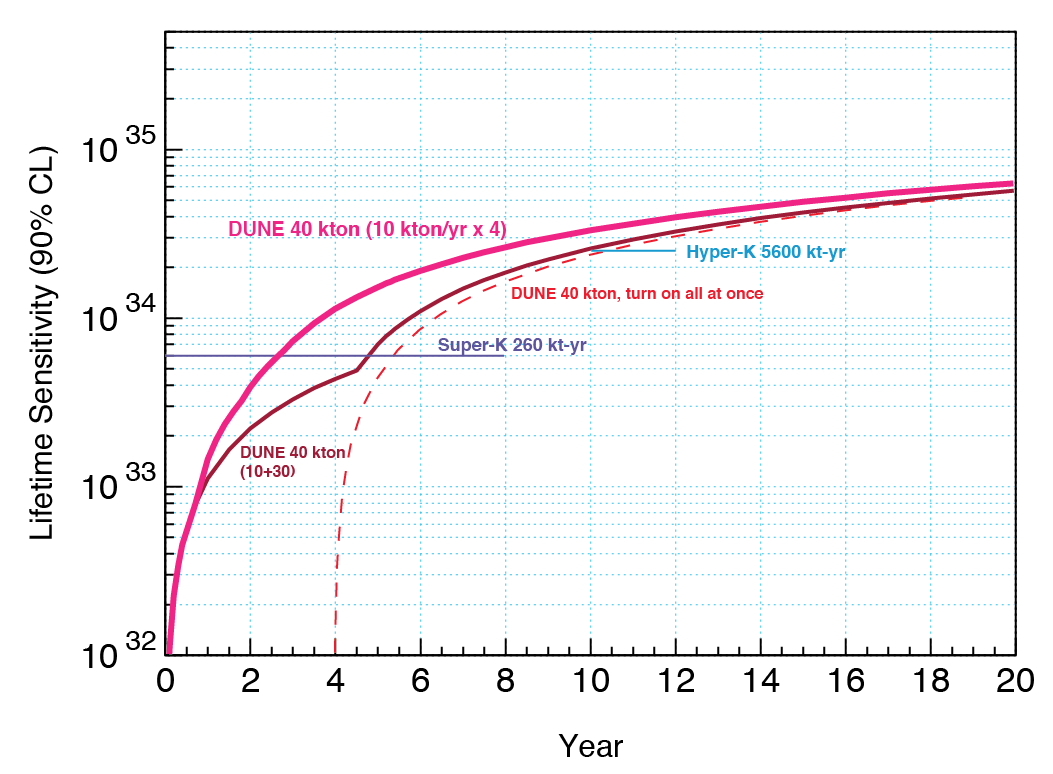
\includegraphics[width=0.8\textwidth]{volume-physics/figures/lar4x10.png}
\end{cdrfigure}

Supersymmetric GUT models in which
the $p\to K^+\overline{\nu}$ channel mode is dominant also favor
other modes involving kaons in the final state, thus enabling a rich 
program of searches for nucleon decay in the DUNE LArTPC detectors.


%%%%%%%%%%%%%%%%%%%%%%%%%%%%%%%%%%%%%%%%%%%%%%%%%%%%%%%%%%%%%%%%%%%%%%%%%%%%%%%%%%
%\paragraph*{Studies of Supernova Neutrino Bursts.}
\section{Supernova-Neutrino Physics and Astrophysics}

The neutrinos from a core-collapse supernova are emitted in a burst of
a few tens of seconds duration, with about half in the first
second. Energies are in the range of a few tens of MeV, and the
luminosity is divided roughly equally between the three known neutrino
flavors.  Currently, experiments worldwide are sensitive primarily to
electron antineutrinos ($\bar{\nu}_e$), with detection through the inverse-beta decay
process on free protons\footnote{This refers to neutrino interactions with the nucleus of a
hydrogen atom in H$_2$O in water detectors or in hydrocarbon chains in 
liquid scintillator detectors.},
 which dominates the interaction rate in water
and liquid-scintillator detectors.  Liquid argon has a unique sensitivity to
the electron-neutrino ($\nu_e$) component of the flux, via the absorption
interaction on $^{40}$Ar as follows:
\begin{eqnarray*}
\nu_e +{}^{40}{\rm Ar} & \rightarrow & e^-+{}^{40}{\rm K^*}
\end{eqnarray*} 
This interaction can be tagged via the coincidence of the emitted
electron and the accompanying photon cascade from the $^{40}{\rm K^*}$
de-excitation.  About \num{3000} events would be expected in a \ktadj{40}
fiducial mass liquid argon detector for a supernova at a distance of
\SI{10}{\kilo\parsec}.  In the neutrino channel the oscillation
features are in general more pronounced, since the $\nu_e$ spectrum is
always significantly different from the $\nu_\mu$ ($\nu_\tau$) spectra
in the initial core-collapse stages, to a larger degree than is the
case for the corresponding $\bar{\nu}_e$ spectrum.  Detection of a large
neutrino signal in DUNE would help provide critical information on key
astrophysical phenomena such as
\begin{itemize}
\item the neutronization burst
\item formation of a black hole
\item shock wave effects
\item shock instability oscillations
\item turbulence effects
\end{itemize}

In addition to providing unprecedented information on the mechanics of
the supernova explosion, observation of a core-collapse supernova in
DUNE will also enable searches for numerous types of new physics
including various Goldstone bosons (e.g., Majorons), neutrino magnetic
moments, new gauge bosons (``dark photons''), ``unparticles'' and
extra-dimensional gauge bosons.

%%%%%%%%%%%%%%%%%%%%%%%%%%%%%%%%%%%%%%%%%%%%%%%%%%%%%%%%%%%%%%%%%%%%%%%%%%%%%%%%%%
%
%
\section{Precision Measurements with a High-Intensity Neutrino Source and High-Resolution Near Detector}

\fixme{Can we shorten the title assuming a near detector is near a source and that source is the lbnf beam (i.e., high-intensity)? I propose: Precision Measurements with High-Resolution Near Detector}

The DUNE near neutrino detector will provide precision measurements of
neutrino interactions, which, in the medium-to-long term, are essential
for controlling the systematic uncertainties in the long-baseline
oscillation physics program.  The near detector %, which will include argon targets, 
will include argon targets and will measure the absolute flux and energy-dependent
shape of all four neutrino species, \numu, \anumu, \nue and \anue,
%$\nu_\mu$, $\bar{\nu}_{\mu}$,$\nu_e$ and $\bar{\nu}_e$, 
to accurately predict for each species the
far/near flux ratio as a function of energy.  It will also measure the
four-momenta of secondary hadrons, such as charged and neutral mesons,
produced in the neutral and charged current interactions that
constitute the dominant backgrounds to the oscillation signals.

With  \num{240000} (\num{85000}) %$\nu_\mu$ ($\overline{\nu}_\mu$) 
\numu (\anumu) charged current 
and \num{90000} (\num{35000})  neutral current interactions per ton per \num{1e20} %$1 \times 10^{20}$
protons-on-target at \SI{120}{GeV}  in the $\nu$ ($\overline\nu$) beam, the near detector
will also be the source of data for a rich program of neutrino-interaction 
physics in its own right.  These numbers correspond to
\num{e7}  neutrino interactions per year for the range of beam
configurations and near detector designs under consideration.
Measurement of fluxes, cross sections and particle production over a
large energy range of \SIrange{0.5}{50}{\GeV} (which can also help constrain
backgrounds to proton decay signals from atmospheric neutrinos) are the key
elements of this program.  
Furthermore, since the near detector data will feature very large
samples of events that are amenable to precision reconstruction and
analysis, they can be exploited for sensitive studies of electroweak
physics and nucleon structure, as well as for searches for new physics
in unexplored regions (heavy sterile neutrinos, high-$\Delta m^2$
oscillations, light Dark Matter particles, and so on). 

%Furthermore, since the near detector data will feature very large samples of events that are amenable to precision reconstruction and analysis, theycan be exploited for sensitive studies of electroweak physics andnucleon structure.  

%\clearpage
%%%%%%%%%%%%%%%%%%%%%%%%%%%%%%%%%%%%%%%%%%%%%%%%%%%%%%%%%%%%%%%%%%%%%%%%%%%%%%%%%%
%
\section{Summary}
%\section{Concluding Remarks}


This chapter %has touched 
touches only briefly on the most prominent portion of
the full suite of physics opportunities enabled by DUNE.  
%\fixme{Makes
%  it sound like there are MANY physics topics not mentioned here.} 
\volphys includes a more detailed discussion and covers topics %, as well as topics
that were omitted here in the interest of brevity and focus.  In
Chapter~\ref{v1ch:strategy} progress toward DUNE physics milestones is
addressed, based on potential scenarios for the deployment of DUNE
detector modules, the beamline and PIP-II implementations. 
%The present chapter concludes with a summary of its key points.

In summary, the primary science goals of DUNE are drivers for the advancement of
particle physics. The questions being addressed are of wide-ranging
consequence: the origin of flavor and the generation structure of the
fermions (i.e., the existence of three families of quark and lepton
flavors), the physical mechanism that provides the CP violation needed
to generate the Baryon Asymmetry of the Universe (BAU), and the high-energy
physics that would lead to the instability of matter.  Achieving these
goals requires a dedicated, ambitious and long-term program.  No other
proposed long-baseline neutrino oscillation program with the
scientific scope and sensitivity of DUNE is as advanced in terms of
engineering development and project planning.  Implementation of a
staged program with a far detector of even modest size in the initial
stage (e.g., \SI{10}\kt) will enable exciting physics in the intermediate
term, including a definitive mass hierarchy determination and a
measurement of the CP phase without ambiguities, while providing the
fastest route toward achieving the full range of DUNE's science
objectives.  Should DUNE find that the CP phase is not zero or $\pi$,
it will have found strong indications ($>3\sigma$) of leptonic CP
violation.

The DUNE experiment is a world-leading international physics
experiment, bringing together the %world's 
global neutrino community as well
as leading experts in nucleon decay and particle astrophysics to
explore key questions at the forefront of particle physics and
astrophysics. The highly capable beam and detectors will enable a
large suite of new physics measurements with potential groundbreaking
discoveries.

%%%%%%%%%%%%%%%%%%%%%%%%%%%%%%%%%%%%%%%%%%%%%%%%%%%%%%%%%%%%%%%%%%%%%%%%%%%%%%%%%%
%%%%%%%%%%%%%%%%%%%%%%%%%%%%%%%%%%%%%%%%%%%%%%%%%%%%%%%%%%%%%%%%%%%%%%%%%%%%%%%%%%
%\begin{thebibliography}{99}


%\bibitem{snowmass2013} APS Division of Particles and Fields 
%        Community Summer Study 2013, 
%        \url{http://www.snowmass2013.org/}.

%\bibitem{cdzero} DOE Office of Science, Office of High Energy Physics, ``Mission 
%         Need Statement for a Long Baseline Neutrino Experiment (LBNE) Major
%         System'', LBNE-doc-6259, September 2009, 
%         \url{http://lbne2-docdb.fnal.gov/cgi-bin/ShowDocument?docid=6259}. 

%\bibitem{nusandbeyond} ``Neutrinos and Beyond: New Windows on Nature'', 
%                The NRC Neutrino Facilities Assessment Committee, 
%                The National Academies Press, ISBN 0-309-08716-3, (2003).

%\bibitem{potu} ``The Physics of the Universe, a Strategic Plan for Federal Research at
%		the Intersection of Physics and Astronomy", 
%		National Science and Technology Council Committee on Science, February 2004,
%		\url{http://www.ostp.gov/html/physicsoftheuniverse2.pdf}.

%\bibitem{epp2010} ``Revealing the Hidden Nature of Space and Time: Charting the 
%                Course for Elementary Particle Physics'', The National Academies 
%                Press, ISBN 0-309-66039-4, (2006).

%\bibitem{nusag} ``Recommendations to the Department of Energy and the National 
%                Science Foundation on a Future U.S. Program in Neutrino 
%                Oscillations'', report of the HEPAP/NSAC 
%                Neutrino Scientific Assessment Group, July 2007.

%\bibitem{p5report} Particle Physics Project Prioritization Panel, ``U.S. Particle 
%         Physics: Scientific opportunities, a plan for the next ten years'', May 
%         2008,  \url{http://www.er.doe.gov/hep/files/pdfs/P5_Report 06022008.pdf}.

%\bibitem{nasdusel} ``An Assessment of the Deep Underground Science and 
%                   Engineering Laboratory'', The National Academies Press, 
%                   ISBN 978-0-309-2172three-1, (2012).

%\bibitem{facilitiesreport} ``Input to the prioritization of proposed scientific 
%                            user facilities for the Office of Science'', 
%                            HEPAP Facilities Subpanel, March 2013.

%\bibitem{pxbook} A. S. Kronfeld and R. S. Tschirhart, eds., 
%                 ``Project X: Physics Opportunities'', July 2013, 
%                 \url{http://projectx-docdb.fnal.gov/cgi-bin/ShowDocument?docid=1199}.

%\bibitem{snowmass-neutrino} A.\ de Gouvea {\sl et al.}, ``Neutrinos'',  
%                            Intensity Frontier Working Group Report, DPF Community 
%                            Summer Study 2013, posted at
%                            \url{http://www.snowmass2013.org/tiki-index.php?page=Neutrinos}.

%\bibitem{snowmass-baryon} K. S. Babu and E. Kearns, eds., ``Baryon Number Violation'', 
%                          Intensity Frontier Working Group report, DPF Community 
%                          Summer Study 2013.  See 
%                          \url{http://www.snowmass2013.org/tiki-index.php?page=Baryon+Number+Violation}.

%\bibitem{mar2012review} Final Report, Director's Independent Conceptual Design 
%                        and CD-1 Readiness Review of the LBNE Project, March 2012,
%                        \url{http://lbne2-docdb.fnal.gov:8080/0057/005788/003/FinalReportDirector%27sReviewLBNE2012-0three-30.pdf}
%
%\bibitem{LBNEreconfig} Y.-K. Kim {\sl et al.}, 
%        LBNE Reconfiguration Steering Committee Report, August 2012, see
%        \url{http://www.fnal.gov/directorate/lbne_reconfiguration/index.shtml}.
%        See also, J. Appel {\sl et al.}, ``Physics Working Group Report to 
%        the LBNE Reconfiguration Steering Committee'', also posted at the above URL.

%\bibitem{cdr} LBNE Conceptual Design Report, October 2012, see  
%         \url{https://sharepoint.fnal.gov/project/lbne/LBNE\%20at\%20Work/SitePages/Reports\%20and\%20Documents.aspx}.

%\bibitem{cd1document} DOE Office of Science, Office of High Energy Physics, 
%                      ``Critical Decision 1: Approve Alternate Selection and 
%                      Cost Range of the Long Baseline Neutrino Experiment 
%                      (LBNE) Project at the Fermi National Accelerator 
%                      Laboratory and Sanford Underground Research Facility'',
%                      LBNE-doc-6681, December 2012, 
%         \url{http://lbne2-docdb.fnal.gov/cgi-bin/ShowDocument?docid=6681}.
%        see also LBNE-doc-6963

%\bibitem{europeanstrategy} The European Strategy for Particle Physics, Update 2013, 
%        CERN-Council-S/106, 7 May 2013, 
%        \url{http://council.web.cern.ch/council/en/EuropeanStrategy/ESParticlePhysics.html}.

%\bibitem{wilson-fermilab-pac} R.~J.~Wilson, ``LBNE Collaboration Status'', 
%       presentation to the Fermilab Program Advisory Committee, June 2013, 
%       \url{http://www.fnal.gov/directorate/program_planning/June2013PACPublic/LBNECollabStat%us_PAC_June2013.pdf}.

%\bibitem{docdb-3056} The LBNE Project, ``Physics Research Goals of the LBNE 
%         Project'', LBNE-doc-3056v8, January 2013,
%         \url{http://lbne2-docdb.fnal.gov/cgi-bin/ShowDocument?docid=3056}.
%         
%\bibitem{Akiri:2011dv} T. Akiri {\sl et al.} (LBNE Collaboration), ``The 2010 Interim 
%         Report of the Long-Baseline Neutrino Expeirment Collaboration Physics 
%         Working Groups'', arXiv:1110.6249 [hep-ex], 2011.

%\bibitem{extendednova} M. Messier, for the NOvA Collaboration, ``Extending the 
%                       NOvA Physics Program'', Whitepaper submitted to the 
%                       Neutrino Working Group of the DPF Community Summer Study 2013, 
%                       January 2013, 
%                       \url{http://if-neutrino.fnal.gov/whitepapers/messier-nova.pdf}

%\bibitem{t2k} K. Abe {\sl et al.} (T2K Collaboration), Phys.\ Rev.\ Lett.\ \textbf{ 107}, 
%              041801 (2011).

%\bibitem{MINOS-nue} P. Adamson {\sl et al.} (MINOS Collaboration), 
%                   Phys.\ Rev.\ Lett. \textbf{ 107}, 181802 (2011).

%\bibitem{dchooz} Y. Abe {\sl et al.} (Double Chooz Collaboration), Phys.\ Rev.\ D \textbf{ 86}, 
%                 052008 (2012).

%\bibitem{dayabay} F. P. An {\sl et. al} (Daya Bay Collaboration), 
%                  Phys.\ Rev.\ Lett.\ \textbf{ 108}, 171803 (2012).
%                 arXiv:1203.1669 [hep-ex]

%\bibitem{reno} J. Ahn {\sl et al.} (RENO Collaboration), Phys.\ Rev.\ Lett.\ \textbf{ 108},
%               191802 (2012).

%\bibitem{Huber:2010dx} P. Huber and J. Kopp, JHEP \textbf{ 1103}, 013 (2011).

%\bibitem{kearns-isoups} E. Kearns, ``Future Experiments for Proton Decay'', 
%                        presentation at ISOUPS (International Symposium:
%                        Opportunities in Underground Physics for Snowmass), Asilomar, 
%                        May 2013.

%\end{thebibliography}

%\end{document}
